\mbox{$\displaystyle -\,$\,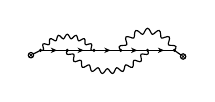
\begin{tikzpicture}[x=0.340cm, y=0.340cm, line width=0.420pt, baseline={([yshift=-0.6ex]0,0)}]
  \draw (-0.500,0.000) -- (0.500,0.000);
  \fill (0.119,0.000) -- (-0.119,0.102) -- (-0.042,0.000) -- (-0.119,-0.102) -- cycle;
  \draw (-1.500,0.000) -- (-0.500,0.000);
  \fill (-0.881,0.000) -- (-1.119,0.102) -- (-1.042,0.000) -- (-1.119,-0.102) -- cycle;
  \draw (0.500,0.000) -- (1.500,0.000);
  \fill (1.119,0.000) -- (0.881,0.102) -- (0.958,0.000) -- (0.881,-0.102) -- cycle;
  \draw (-2.500,0.000) -- (-1.500,0.000);
  \fill (-1.881,0.000) -- (-2.119,0.102) -- (-2.042,0.000) -- (-2.119,-0.102) -- cycle;
  \draw (1.500,0.000) -- (2.500,0.000);
  \fill (2.119,0.000) -- (1.881,0.102) -- (1.958,0.000) -- (1.881,-0.102) -- cycle;
  \draw plot[smooth, tension=0.7] coordinates {(0.500,0.000) (0.448,0.075) (0.440,0.137) (0.492,0.174) (0.582,0.185) (0.671,0.188) (0.722,0.210) (0.725,0.265) (0.698,0.350) (0.678,0.439) (0.694,0.500) (0.756,0.514) (0.844,0.491) (0.927,0.461) (0.983,0.462) (1.006,0.512) (1.013,0.601) (1.027,0.691) (1.066,0.741) (1.128,0.731) (1.200,0.677) (1.267,0.617) (1.319,0.597) (1.359,0.635) (1.399,0.715) (1.446,0.793) (1.500,0.825) (1.554,0.793) (1.601,0.715) (1.641,0.635) (1.681,0.597) (1.733,0.617) (1.800,0.677) (1.872,0.731) (1.934,0.741) (1.973,0.691) (1.987,0.601) (1.994,0.512) (2.017,0.462) (2.073,0.461) (2.156,0.491) (2.244,0.514) (2.306,0.500) (2.322,0.439) (2.302,0.350) (2.275,0.265) (2.278,0.210) (2.329,0.188) (2.418,0.185) (2.508,0.174) (2.560,0.137) (2.552,0.075) (2.500,0.000)};
  \draw plot[smooth, tension=0.7] coordinates {(-0.500,0.000) (-0.569,-0.003) (-0.610,0.012) (-0.615,0.055) (-0.598,0.122) (-0.583,0.190) (-0.596,0.236) (-0.642,0.247) (-0.710,0.230) (-0.776,0.210) (-0.820,0.214) (-0.836,0.254) (-0.835,0.323) (-0.839,0.393) (-0.862,0.434) (-0.910,0.433) (-0.971,0.400) (-1.030,0.363) (-1.073,0.356) (-1.099,0.391) (-1.116,0.458) (-1.137,0.525) (-1.170,0.559) (-1.216,0.546) (-1.267,0.498) (-1.315,0.448) (-1.355,0.429) (-1.389,0.457) (-1.422,0.518) (-1.459,0.577) (-1.500,0.601) (-1.541,0.577) (-1.578,0.518) (-1.611,0.457) (-1.645,0.429) (-1.685,0.448) (-1.733,0.498) (-1.784,0.546) (-1.830,0.559) (-1.863,0.525) (-1.884,0.458) (-1.901,0.391) (-1.927,0.356) (-1.970,0.363) (-2.029,0.400) (-2.090,0.433) (-2.138,0.434) (-2.161,0.393) (-2.165,0.323) (-2.164,0.254) (-2.180,0.214) (-2.224,0.210) (-2.290,0.230) (-2.358,0.247) (-2.404,0.236) (-2.417,0.190) (-2.402,0.122) (-2.385,0.055) (-2.390,0.012) (-2.431,-0.003) (-2.500,0.000)};
  \draw plot[smooth, tension=0.7] coordinates {(1.500,0.000) (1.528,-0.078) (1.521,-0.133) (1.469,-0.154) (1.386,-0.146) (1.305,-0.135) (1.255,-0.148) (1.244,-0.199) (1.259,-0.279) (1.270,-0.361) (1.252,-0.414) (1.197,-0.424) (1.118,-0.399) (1.041,-0.372) (0.988,-0.375) (0.968,-0.423) (0.966,-0.505) (0.961,-0.587) (0.933,-0.636) (0.877,-0.634) (0.804,-0.594) (0.734,-0.552) (0.682,-0.544) (0.652,-0.587) (0.634,-0.667) (0.612,-0.747) (0.575,-0.788) (0.521,-0.775) (0.458,-0.722) (0.397,-0.667) (0.348,-0.649) (0.310,-0.685) (0.276,-0.759) (0.239,-0.833) (0.194,-0.866) (0.144,-0.843) (0.092,-0.778) (0.045,-0.711) (0.000,-0.684) (-0.045,-0.711) (-0.092,-0.778) (-0.144,-0.843) (-0.194,-0.866) (-0.239,-0.833) (-0.276,-0.759) (-0.310,-0.685) (-0.348,-0.649) (-0.397,-0.667) (-0.458,-0.722) (-0.521,-0.775) (-0.575,-0.788) (-0.612,-0.747) (-0.634,-0.667) (-0.652,-0.587) (-0.682,-0.544) (-0.734,-0.552) (-0.804,-0.594) (-0.877,-0.634) (-0.933,-0.636) (-0.961,-0.587) (-0.966,-0.505) (-0.968,-0.423) (-0.988,-0.375) (-1.041,-0.372) (-1.118,-0.399) (-1.197,-0.424) (-1.252,-0.414) (-1.270,-0.361) (-1.259,-0.279) (-1.244,-0.199) (-1.255,-0.148) (-1.305,-0.135) (-1.386,-0.146) (-1.469,-0.154) (-1.521,-0.133) (-1.528,-0.078) (-1.500,0.000)};
  \draw (-2.500,0.000) -- (-2.857,-0.181);
  \draw[fill=white] (-2.857,-0.181) circle (0.100);
  \draw[line width=0.298pt] (-2.787,-0.111) -- (-2.927,-0.251) (-2.787,-0.251) -- (-2.927,-0.111);
  \draw (2.500,0.000) -- (2.828,-0.230);
  \draw[fill=white] (2.828,-0.230) circle (0.100);
  \draw[line width=0.298pt] (2.898,-0.160) -- (2.758,-0.300) (2.898,-0.300) -- (2.758,-0.160);
  \fill (0.500,0.000) circle (0.064);
  \fill (-0.500,0.000) circle (0.064);
  \fill (1.500,0.000) circle (0.064);
  \fill (-1.500,0.000) circle (0.064);
  \fill (2.500,0.000) circle (0.064);
  \fill (-2.500,0.000) circle (0.064);
\end{tikzpicture}}
\diagramgap
\mbox{$\displaystyle -\,$\,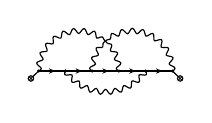
\begin{tikzpicture}[x=0.340cm, y=0.340cm, line width=0.420pt, baseline={([yshift=-0.6ex]0,0)}]
  \draw (-1.500,0.000) -- (-0.500,0.000);
  \fill (-0.881,0.000) -- (-1.119,0.102) -- (-1.042,0.000) -- (-1.119,-0.102) -- cycle;
  \draw (-0.500,0.000) -- (0.500,0.000);
  \fill (0.119,0.000) -- (-0.119,0.102) -- (-0.042,0.000) -- (-0.119,-0.102) -- cycle;
  \draw (0.500,0.000) -- (1.500,0.000);
  \fill (1.119,0.000) -- (0.881,0.102) -- (0.958,0.000) -- (0.881,-0.102) -- cycle;
  \draw (-2.500,0.000) -- (-1.500,0.000);
  \fill (-1.881,0.000) -- (-2.119,0.102) -- (-2.042,0.000) -- (-2.119,-0.102) -- cycle;
  \draw (1.500,0.000) -- (2.500,0.000);
  \fill (2.119,0.000) -- (1.881,0.102) -- (1.958,0.000) -- (1.881,-0.102) -- cycle;
  \draw plot[smooth, tension=0.7] coordinates {(-0.500,0.000) (-0.569,0.049) (-0.595,0.100) (-0.562,0.148) (-0.488,0.188) (-0.413,0.224) (-0.377,0.263) (-0.396,0.312) (-0.453,0.373) (-0.507,0.438) (-0.520,0.494) (-0.477,0.532) (-0.395,0.552) (-0.313,0.568) (-0.269,0.597) (-0.275,0.650) (-0.314,0.723) (-0.351,0.799) (-0.349,0.856) (-0.298,0.882) (-0.214,0.882) (-0.136,0.881) (-0.101,0.911) (-0.098,0.968) (-0.093,1.027) (-0.068,1.068) (-0.029,1.096) (0.008,1.125) (0.044,1.156) (0.091,1.172) (0.143,1.179) (0.182,1.204) (0.196,1.266) (0.203,1.348) (0.230,1.400) (0.288,1.398) (0.361,1.357) (0.432,1.313) (0.484,1.304) (0.515,1.346) (0.536,1.427) (0.562,1.507) (0.603,1.548) (0.658,1.532) (0.719,1.473) (0.776,1.413) (0.824,1.391) (0.865,1.424) (0.906,1.497) (0.951,1.569) (1.000,1.598) (1.049,1.569) (1.094,1.497) (1.135,1.424) (1.176,1.391) (1.224,1.413) (1.281,1.473) (1.342,1.532) (1.397,1.548) (1.438,1.507) (1.464,1.427) (1.485,1.346) (1.516,1.304) (1.568,1.313) (1.639,1.357) (1.712,1.398) (1.770,1.400) (1.799,1.351) (1.804,1.266) (1.804,1.183) (1.824,1.134) (1.877,1.130) (1.956,1.156) (2.038,1.177) (2.094,1.165) (2.110,1.110) (2.093,1.027) (2.073,0.946) (2.080,0.894) (2.130,0.877) (2.214,0.882) (2.298,0.882) (2.349,0.856) (2.351,0.799) (2.314,0.723) (2.275,0.650) (2.269,0.597) (2.313,0.568) (2.395,0.552) (2.477,0.532) (2.520,0.494) (2.507,0.438) (2.453,0.373) (2.396,0.312) (2.377,0.263) (2.413,0.224) (2.488,0.188) (2.562,0.148) (2.595,0.100) (2.569,0.049) (2.500,0.000)};
  \draw plot[smooth, tension=0.7] coordinates {(0.500,0.000) (0.430,0.045) (0.399,0.088) (0.424,0.135) (0.488,0.188) (0.550,0.245) (0.570,0.299) (0.532,0.342) (0.453,0.373) (0.374,0.399) (0.333,0.433) (0.346,0.485) (0.395,0.552) (0.440,0.623) (0.446,0.680) (0.398,0.712) (0.314,0.723) (0.231,0.728) (0.184,0.751) (0.183,0.804) (0.214,0.882) (0.234,0.957) (0.211,1.002) (0.153,1.016) (0.093,1.027) (0.053,1.053) (0.025,1.091) (-0.008,1.125) (-0.044,1.156) (-0.071,1.198) (-0.094,1.248) (-0.132,1.277) (-0.196,1.266) (-0.270,1.234) (-0.325,1.229) (-0.350,1.275) (-0.361,1.357) (-0.377,1.440) (-0.412,1.486) (-0.468,1.477) (-0.536,1.427) (-0.601,1.374) (-0.651,1.358) (-0.688,1.396) (-0.719,1.473) (-0.755,1.550) (-0.800,1.585) (-0.852,1.562) (-0.906,1.497) (-0.955,1.430) (-1.000,1.402) (-1.045,1.430) (-1.094,1.497) (-1.148,1.562) (-1.200,1.585) (-1.245,1.550) (-1.281,1.473) (-1.312,1.396) (-1.349,1.358) (-1.399,1.374) (-1.464,1.427) (-1.532,1.477) (-1.588,1.486) (-1.623,1.440) (-1.639,1.357) (-1.650,1.275) (-1.675,1.229) (-1.728,1.231) (-1.804,1.266) (-1.882,1.298) (-1.939,1.293) (-1.962,1.240) (-1.956,1.156) (-1.946,1.073) (-1.960,1.022) (-2.012,1.012) (-2.093,1.027) (-2.177,1.038) (-2.231,1.019) (-2.240,0.962) (-2.214,0.882) (-2.183,0.804) (-2.184,0.751) (-2.231,0.728) (-2.314,0.723) (-2.398,0.712) (-2.446,0.680) (-2.440,0.623) (-2.395,0.552) (-2.346,0.485) (-2.333,0.433) (-2.374,0.399) (-2.453,0.373) (-2.532,0.342) (-2.570,0.299) (-2.550,0.245) (-2.488,0.188) (-2.424,0.135) (-2.399,0.088) (-2.430,0.045) (-2.500,0.000)};
  \draw plot[smooth, tension=0.7] coordinates {(1.500,0.000) (1.528,-0.078) (1.521,-0.133) (1.469,-0.154) (1.386,-0.146) (1.305,-0.135) (1.255,-0.148) (1.244,-0.199) (1.259,-0.279) (1.270,-0.361) (1.252,-0.414) (1.197,-0.424) (1.118,-0.399) (1.041,-0.372) (0.988,-0.375) (0.968,-0.423) (0.966,-0.505) (0.961,-0.587) (0.933,-0.636) (0.877,-0.634) (0.804,-0.594) (0.734,-0.552) (0.682,-0.544) (0.652,-0.587) (0.634,-0.667) (0.612,-0.747) (0.575,-0.788) (0.521,-0.775) (0.458,-0.722) (0.397,-0.667) (0.348,-0.649) (0.310,-0.685) (0.276,-0.759) (0.239,-0.833) (0.194,-0.866) (0.144,-0.843) (0.092,-0.778) (0.045,-0.711) (0.000,-0.684) (-0.045,-0.711) (-0.092,-0.778) (-0.144,-0.843) (-0.194,-0.866) (-0.239,-0.833) (-0.276,-0.759) (-0.310,-0.685) (-0.348,-0.649) (-0.397,-0.667) (-0.458,-0.722) (-0.521,-0.775) (-0.575,-0.788) (-0.612,-0.747) (-0.634,-0.667) (-0.652,-0.587) (-0.682,-0.544) (-0.734,-0.552) (-0.804,-0.594) (-0.877,-0.634) (-0.933,-0.636) (-0.961,-0.587) (-0.966,-0.505) (-0.968,-0.423) (-0.988,-0.375) (-1.041,-0.372) (-1.118,-0.399) (-1.197,-0.424) (-1.252,-0.414) (-1.270,-0.361) (-1.259,-0.279) (-1.244,-0.199) (-1.255,-0.148) (-1.305,-0.135) (-1.386,-0.146) (-1.469,-0.154) (-1.521,-0.133) (-1.528,-0.078) (-1.500,0.000)};
  \draw (-2.500,0.000) -- (-2.787,-0.278);
  \draw[fill=white] (-2.787,-0.278) circle (0.100);
  \draw[line width=0.298pt] (-2.717,-0.208) -- (-2.857,-0.348) (-2.717,-0.348) -- (-2.857,-0.208);
  \draw (2.500,0.000) -- (2.787,-0.278);
  \draw[fill=white] (2.787,-0.278) circle (0.100);
  \draw[line width=0.298pt] (2.857,-0.208) -- (2.717,-0.348) (2.857,-0.348) -- (2.717,-0.208);
  \fill (-0.500,0.000) circle (0.064);
  \fill (0.500,0.000) circle (0.064);
  \fill (1.500,0.000) circle (0.064);
  \fill (-1.500,0.000) circle (0.064);
  \fill (2.500,0.000) circle (0.064);
  \fill (-2.500,0.000) circle (0.064);
\end{tikzpicture}}
\diagramgap
\mbox{$\displaystyle +\,\frac{1}{6}$\,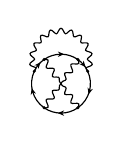
\begin{tikzpicture}[x=0.340cm, y=0.340cm, line width=0.420pt, baseline={([yshift=-0.6ex]0,0)}]
  \draw (-0.631,0.901) arc[start angle=125.000, end angle=55.000, radius=1.100];
  \fill (0.119,1.100) -- (-0.119,1.202) -- (-0.042,1.100) -- (-0.119,0.998) -- cycle;
  \draw (0.631,0.901) arc[start angle=55.000, end angle=25.000, radius=1.100];
  \fill (0.919,0.616) -- (0.844,0.864) -- (0.816,0.739) -- (0.688,0.733) -- cycle;
  \draw (-0.997,0.465) arc[start angle=155.000, end angle=125.000, radius=1.100];
  \fill (-0.766,0.799) -- (-0.998,0.681) -- (-0.870,0.675) -- (-0.841,0.550) -- cycle;
  \draw (0.631,-0.901) arc[start angle=305.000, end angle=235.000, radius=1.100];
  \fill (-0.119,-1.100) -- (0.119,-1.202) -- (0.042,-1.100) -- (0.119,-0.998) -- cycle;
  \draw (0.997,0.465) arc[start angle=25.000, end angle=-55.000, radius=1.100];
  \fill (1.032,-0.400) -- (1.192,-0.196) -- (1.073,-0.244) -- (0.995,-0.143) -- cycle;
  \draw (-0.631,-0.901) arc[start angle=235.000, end angle=155.000, radius=1.100];
  \fill (-1.093,-0.169) -- (-1.130,-0.426) -- (-1.052,-0.325) -- (-0.933,-0.374) -- cycle;
  \draw plot[smooth, tension=0.7] coordinates {(0.631,0.901) (0.665,0.816) (0.662,0.757) (0.607,0.734) (0.516,0.737) (0.425,0.740) (0.370,0.717) (0.368,0.658) (0.402,0.573) (0.435,0.489) (0.433,0.430) (0.378,0.407) (0.287,0.410) (0.196,0.412) (0.141,0.390) (0.138,0.330) (0.172,0.246) (0.192,0.171) (0.166,0.128) (0.110,0.106) (0.057,0.082) (0.025,0.043) (0.000,0.000) (-0.032,-0.039) (-0.057,-0.082) (-0.063,-0.139) (-0.063,-0.200) (-0.095,-0.239) (-0.172,-0.246) (-0.263,-0.243) (-0.318,-0.266) (-0.321,-0.325) (-0.287,-0.410) (-0.253,-0.494) (-0.256,-0.553) (-0.310,-0.576) (-0.402,-0.573) (-0.493,-0.571) (-0.547,-0.593) (-0.550,-0.652) (-0.516,-0.737) (-0.482,-0.822) (-0.485,-0.881) (-0.540,-0.904) (-0.631,-0.901)};
  \draw plot[smooth, tension=0.7] coordinates {(0.997,0.465) (0.950,0.532) (0.938,0.582) (0.977,0.615) (1.055,0.641) (1.131,0.674) (1.168,0.719) (1.146,0.772) (1.081,0.825) (1.015,0.872) (0.986,0.915) (1.012,0.959) (1.076,1.010) (1.138,1.067) (1.157,1.121) (1.118,1.164) (1.040,1.192) (0.961,1.215) (0.920,1.245) (0.930,1.296) (0.973,1.365) (1.011,1.439) (1.011,1.497) (0.960,1.524) (0.877,1.524) (0.795,1.519) (0.746,1.534) (0.738,1.585) (0.756,1.665) (0.767,1.747) (0.748,1.801) (0.691,1.810) (0.612,1.782) (0.537,1.750) (0.486,1.747) (0.461,1.793) (0.450,1.874) (0.434,1.956) (0.397,2.000) (0.341,1.989) (0.276,1.936) (0.216,1.880) (0.168,1.861) (0.130,1.895) (0.093,1.968) (0.049,2.039) (0.000,2.069) (-0.049,2.039) (-0.093,1.968) (-0.130,1.895) (-0.168,1.861) (-0.216,1.880) (-0.276,1.936) (-0.341,1.989) (-0.397,2.000) (-0.434,1.956) (-0.450,1.874) (-0.461,1.793) (-0.486,1.747) (-0.537,1.750) (-0.612,1.782) (-0.691,1.810) (-0.748,1.801) (-0.767,1.747) (-0.756,1.665) (-0.738,1.585) (-0.746,1.534) (-0.795,1.519) (-0.877,1.524) (-0.960,1.524) (-1.011,1.497) (-1.011,1.439) (-0.973,1.365) (-0.930,1.296) (-0.920,1.245) (-0.961,1.215) (-1.040,1.192) (-1.118,1.164) (-1.157,1.121) (-1.138,1.067) (-1.076,1.010) (-1.012,0.959) (-0.986,0.915) (-1.015,0.872) (-1.081,0.825) (-1.146,0.772) (-1.168,0.719) (-1.131,0.674) (-1.055,0.641) (-0.977,0.615) (-0.938,0.582) (-0.950,0.532) (-0.997,0.465)};
  \draw plot[smooth, tension=0.7] coordinates {(-0.631,0.901) (-0.540,0.904) (-0.485,0.881) (-0.482,0.822) (-0.516,0.737) (-0.550,0.652) (-0.547,0.593) (-0.493,0.571) (-0.402,0.573) (-0.310,0.576) (-0.256,0.553) (-0.253,0.494) (-0.287,0.410) (-0.321,0.325) (-0.318,0.266) (-0.263,0.243) (-0.172,0.246) (-0.095,0.239) (-0.063,0.200) (-0.063,0.139) (-0.057,0.082) (-0.032,0.039) (0.000,0.000) (0.025,-0.043) (0.057,-0.082) (0.110,-0.106) (0.166,-0.128) (0.192,-0.171) (0.172,-0.246) (0.138,-0.330) (0.141,-0.390) (0.196,-0.412) (0.287,-0.410) (0.378,-0.407) (0.433,-0.430) (0.435,-0.489) (0.402,-0.573) (0.368,-0.658) (0.370,-0.717) (0.425,-0.740) (0.516,-0.737) (0.607,-0.734) (0.662,-0.757) (0.665,-0.816) (0.631,-0.901)};
  \fill (0.631,0.901) circle (0.064);
  \fill (0.997,0.465) circle (0.064);
  \fill (-0.631,0.901) circle (0.064);
  \fill (-0.631,-0.901) circle (0.064);
  \fill (0.631,-0.901) circle (0.064);
  \fill (-0.997,0.465) circle (0.064);
\end{tikzpicture}}
\diagramgap
\mbox{$\displaystyle +\,\frac{1}{2}$\,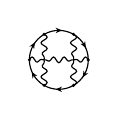
\begin{tikzpicture}[x=0.340cm, y=0.340cm, line width=0.420pt, baseline={([yshift=-0.6ex]0,0)}]
  \draw (-1.100,0.000) arc[start angle=180.000, end angle=120.000, radius=1.100];
  \fill (-0.893,0.653) -- (-1.101,0.498) -- (-0.974,0.514) -- (-0.924,0.396) -- cycle;
  \draw (-0.550,0.953) arc[start angle=120.000, end angle=60.000, radius=1.100];
  \fill (0.119,1.100) -- (-0.119,1.202) -- (-0.042,1.100) -- (-0.119,0.998) -- cycle;
  \draw (-0.550,-0.953) arc[start angle=240.000, end angle=180.000, radius=1.100];
  \fill (-1.012,-0.447) -- (-0.981,-0.704) -- (-0.932,-0.586) -- (-0.805,-0.602) -- cycle;
  \draw (0.550,-0.953) arc[start angle=300.000, end angle=240.000, radius=1.100];
  \fill (-0.119,-1.100) -- (0.119,-1.202) -- (0.042,-1.100) -- (0.119,-0.998) -- cycle;
  \draw (0.550,0.953) arc[start angle=60.000, end angle=0.000, radius=1.100];
  \fill (1.012,0.447) -- (0.981,0.704) -- (0.932,0.586) -- (0.805,0.602) -- cycle;
  \draw (1.100,0.000) arc[start angle=0.000, end angle=-60.000, radius=1.100];
  \fill (0.893,-0.653) -- (1.101,-0.498) -- (0.974,-0.514) -- (0.924,-0.396) -- cycle;
  \draw plot[smooth, tension=0.7] coordinates {(-0.550,0.953) (-0.469,0.900) (-0.436,0.847) (-0.469,0.794) (-0.550,0.741) (-0.631,0.688) (-0.664,0.635) (-0.631,0.582) (-0.550,0.529) (-0.469,0.476) (-0.436,0.423) (-0.469,0.370) (-0.550,0.318) (-0.613,0.265) (-0.617,0.212) (-0.580,0.159) (-0.550,0.106) (-0.546,0.053) (-0.550,0.000) (-0.546,-0.053) (-0.550,-0.106) (-0.580,-0.159) (-0.617,-0.212) (-0.613,-0.265) (-0.550,-0.318) (-0.469,-0.370) (-0.436,-0.423) (-0.469,-0.476) (-0.550,-0.529) (-0.631,-0.582) (-0.664,-0.635) (-0.631,-0.688) (-0.550,-0.741) (-0.469,-0.794) (-0.436,-0.847) (-0.469,-0.900) (-0.550,-0.953)};
  \draw plot[smooth, tension=0.7] coordinates {(0.550,0.953) (0.631,0.900) (0.664,0.847) (0.631,0.794) (0.550,0.741) (0.469,0.688) (0.436,0.635) (0.469,0.582) (0.550,0.529) (0.631,0.476) (0.664,0.423) (0.631,0.370) (0.550,0.318) (0.487,0.265) (0.483,0.212) (0.520,0.159) (0.550,0.106) (0.554,0.053) (0.550,0.000) (0.554,-0.053) (0.550,-0.106) (0.520,-0.159) (0.483,-0.212) (0.487,-0.265) (0.550,-0.318) (0.631,-0.370) (0.664,-0.423) (0.631,-0.476) (0.550,-0.529) (0.469,-0.582) (0.436,-0.635) (0.469,-0.688) (0.550,-0.741) (0.631,-0.794) (0.664,-0.847) (0.631,-0.900) (0.550,-0.953)};
  \draw plot[smooth, tension=0.7] coordinates {(-1.100,0.000) (-1.050,0.076) (-1.000,0.108) (-0.950,0.076) (-0.900,0.000) (-0.850,-0.071) (-0.800,-0.084) (-0.750,-0.045) (-0.700,0.000) (-0.650,0.014) (-0.600,0.006) (-0.550,0.000) (-0.500,0.000) (-0.450,-0.014) (-0.400,-0.041) (-0.350,-0.045) (-0.300,0.000) (-0.250,0.071) (-0.200,0.108) (-0.150,0.076) (-0.100,0.000) (-0.050,-0.076) (0.000,-0.108) (0.050,-0.076) (0.100,0.000) (0.150,0.076) (0.200,0.108) (0.250,0.071) (0.300,0.000) (0.350,-0.045) (0.400,-0.041) (0.450,-0.014) (0.500,0.000) (0.550,0.000) (0.600,0.006) (0.650,0.014) (0.700,0.000) (0.750,-0.045) (0.800,-0.084) (0.850,-0.071) (0.900,0.000) (0.950,0.076) (1.000,0.108) (1.050,0.076) (1.100,0.000)};
  \fill (-0.550,0.953) circle (0.064);
  \fill (0.550,0.953) circle (0.064);
  \fill (-1.100,0.000) circle (0.064);
  \fill (-0.550,-0.953) circle (0.064);
  \fill (1.100,0.000) circle (0.064);
  \fill (0.550,-0.953) circle (0.064);
\end{tikzpicture}}
\diagramgap
\mbox{$\displaystyle -\,\frac{1}{6}$\,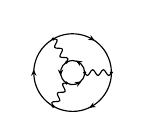
\begin{tikzpicture}[x=0.340cm, y=0.340cm, line width=0.420pt, baseline={([yshift=-0.6ex]0,0)}]
  \draw (-0.725,1.256) arc[start angle=120.000, end angle=0.000, radius=1.450];
  \fill (0.828,1.196) -- (0.673,1.404) -- (0.689,1.277) -- (0.571,1.227) -- cycle;
  \draw (1.450,0.000) arc[start angle=360.000, end angle=240.000, radius=1.450];
  \fill (0.622,-1.315) -- (0.879,-1.284) -- (0.761,-1.235) -- (0.777,-1.108) -- cycle;
  \draw (-0.725,-1.256) arc[start angle=240.000, end angle=120.000, radius=1.450];
  \fill (-1.450,0.119) -- (-1.552,-0.119) -- (-1.450,-0.042) -- (-1.348,-0.119) -- cycle;
  \draw (-0.225,-0.390) arc[start angle=240.000, end angle=360.000, radius=0.450];
  \fill (0.328,-0.330) -- (0.071,-0.361) -- (0.189,-0.411) -- (0.173,-0.538) -- cycle;
  \draw (0.450,0.000) arc[start angle=0.000, end angle=120.000, radius=0.450];
  \fill (0.122,0.449) -- (0.277,0.242) -- (0.261,0.369) -- (0.379,0.418) -- cycle;
  \draw (-0.225,0.390) arc[start angle=120.000, end angle=240.000, radius=0.450];
  \fill (-0.450,-0.119) -- (-0.348,0.119) -- (-0.450,0.042) -- (-0.552,0.119) -- cycle;
  \draw plot[smooth, tension=0.7] coordinates {(1.450,0.000) (1.400,-0.076) (1.350,-0.108) (1.300,-0.076) (1.250,0.000) (1.200,0.076) (1.150,0.108) (1.100,0.076) (1.050,0.000) (1.000,-0.076) (0.950,-0.108) (0.900,-0.076) (0.850,0.000) (0.800,0.076) (0.750,0.108) (0.700,0.076) (0.650,0.000) (0.600,-0.076) (0.550,-0.108) (0.500,-0.076) (0.450,0.000)};
  \draw plot[smooth, tension=0.7] coordinates {(-0.725,-1.256) (-0.766,-1.174) (-0.769,-1.115) (-0.716,-1.088) (-0.625,-1.083) (-0.534,-1.077) (-0.481,-1.050) (-0.484,-0.991) (-0.525,-0.909) (-0.566,-0.828) (-0.569,-0.769) (-0.516,-0.741) (-0.425,-0.736) (-0.334,-0.731) (-0.281,-0.704) (-0.284,-0.644) (-0.325,-0.563) (-0.366,-0.481) (-0.369,-0.422) (-0.316,-0.395) (-0.225,-0.390)};
  \draw plot[smooth, tension=0.7] coordinates {(-0.725,1.256) (-0.634,1.251) (-0.581,1.223) (-0.584,1.164) (-0.625,1.083) (-0.666,1.001) (-0.669,0.942) (-0.616,0.914) (-0.525,0.909) (-0.434,0.904) (-0.381,0.877) (-0.384,0.818) (-0.425,0.736) (-0.466,0.655) (-0.469,0.596) (-0.416,0.568) (-0.325,0.563) (-0.234,0.558) (-0.181,0.530) (-0.184,0.471) (-0.225,0.390)};
  \fill (1.450,0.000) circle (0.064);
  \fill (-0.725,-1.256) circle (0.064);
  \fill (-0.725,1.256) circle (0.064);
  \fill (0.450,0.000) circle (0.064);
  \fill (-0.225,0.390) circle (0.064);
  \fill (-0.225,-0.390) circle (0.064);
\end{tikzpicture}}
\diagramgap
\mbox{$\displaystyle -\,\frac{1}{6}$\,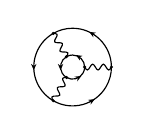
\begin{tikzpicture}[x=0.340cm, y=0.340cm, line width=0.420pt, baseline={([yshift=-0.6ex]0,0)}]
  \draw (-0.725,-1.256) arc[start angle=240.000, end angle=360.000, radius=1.450];
  \fill (0.828,-1.196) -- (0.571,-1.227) -- (0.689,-1.277) -- (0.673,-1.404) -- cycle;
  \draw (1.450,0.000) arc[start angle=0.000, end angle=120.000, radius=1.450];
  \fill (0.622,1.315) -- (0.777,1.108) -- (0.761,1.235) -- (0.879,1.284) -- cycle;
  \draw (-0.725,1.256) arc[start angle=120.000, end angle=240.000, radius=1.450];
  \fill (-1.450,-0.119) -- (-1.348,0.119) -- (-1.450,0.042) -- (-1.552,0.119) -- cycle;
  \draw (-0.225,-0.390) arc[start angle=240.000, end angle=360.000, radius=0.450];
  \fill (0.328,-0.330) -- (0.071,-0.361) -- (0.189,-0.411) -- (0.173,-0.538) -- cycle;
  \draw (0.450,0.000) arc[start angle=0.000, end angle=120.000, radius=0.450];
  \fill (0.122,0.449) -- (0.277,0.242) -- (0.261,0.369) -- (0.379,0.418) -- cycle;
  \draw (-0.225,0.390) arc[start angle=120.000, end angle=240.000, radius=0.450];
  \fill (-0.450,-0.119) -- (-0.348,0.119) -- (-0.450,0.042) -- (-0.552,0.119) -- cycle;
  \draw plot[smooth, tension=0.7] coordinates {(1.450,0.000) (1.400,-0.076) (1.350,-0.108) (1.300,-0.076) (1.250,0.000) (1.200,0.076) (1.150,0.108) (1.100,0.076) (1.050,0.000) (1.000,-0.076) (0.950,-0.108) (0.900,-0.076) (0.850,0.000) (0.800,0.076) (0.750,0.108) (0.700,0.076) (0.650,0.000) (0.600,-0.076) (0.550,-0.108) (0.500,-0.076) (0.450,0.000)};
  \draw plot[smooth, tension=0.7] coordinates {(-0.725,1.256) (-0.634,1.251) (-0.581,1.223) (-0.584,1.164) (-0.625,1.083) (-0.666,1.001) (-0.669,0.942) (-0.616,0.914) (-0.525,0.909) (-0.434,0.904) (-0.381,0.877) (-0.384,0.818) (-0.425,0.736) (-0.466,0.655) (-0.469,0.596) (-0.416,0.568) (-0.325,0.563) (-0.234,0.558) (-0.181,0.530) (-0.184,0.471) (-0.225,0.390)};
  \draw plot[smooth, tension=0.7] coordinates {(-0.725,-1.256) (-0.766,-1.174) (-0.769,-1.115) (-0.716,-1.088) (-0.625,-1.083) (-0.534,-1.077) (-0.481,-1.050) (-0.484,-0.991) (-0.525,-0.909) (-0.566,-0.828) (-0.569,-0.769) (-0.516,-0.741) (-0.425,-0.736) (-0.334,-0.731) (-0.281,-0.704) (-0.284,-0.644) (-0.325,-0.563) (-0.366,-0.481) (-0.369,-0.422) (-0.316,-0.395) (-0.225,-0.390)};
  \fill (1.450,0.000) circle (0.064);
  \fill (-0.725,1.256) circle (0.064);
  \fill (-0.725,-1.256) circle (0.064);
  \fill (0.450,0.000) circle (0.064);
  \fill (-0.225,0.390) circle (0.064);
  \fill (-0.225,-0.390) circle (0.064);
\end{tikzpicture}}
\diagramgap
\mbox{$\displaystyle -\,\frac{1}{2}$\,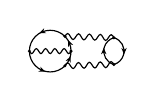
\begin{tikzpicture}[x=0.340cm, y=0.340cm, line width=0.420pt, baseline={([yshift=-0.6ex]0,0)}]
  \draw (-0.639,-0.550) arc[start angle=315.000, end angle=360.000, radius=0.778];
  \fill (-0.425,-0.187) -- (-0.610,-0.369) -- (-0.486,-0.336) -- (-0.422,-0.447) -- cycle;
  \draw (-0.411,0.000) arc[start angle=0.000, end angle=45.000, radius=0.778];
  \fill (-0.516,0.408) -- (-0.519,0.148) -- (-0.454,0.259) -- (-0.330,0.226) -- cycle;
  \draw (-1.967,0.000) arc[start angle=180.000, end angle=315.000, radius=0.778];
  \fill (-1.376,-0.764) -- (-1.558,-0.579) -- (-1.525,-0.703) -- (-1.636,-0.767) -- cycle;
  \draw (-0.639,0.550) arc[start angle=45.000, end angle=180.000, radius=0.778];
  \fill (-1.597,0.673) -- (-1.337,0.670) -- (-1.448,0.735) -- (-1.415,0.859) -- cycle;
  \draw (1.189,-0.500) arc[start angle=254.378, end angle=105.622, radius=0.519];
  \fill (0.810,0.119) -- (0.708,-0.119) -- (0.810,-0.042) -- (0.912,-0.119) -- cycle;
  \draw (1.189,0.500) arc[start angle=74.378, end angle=-74.378, radius=0.519];
  \fill (1.568,-0.119) -- (1.670,0.119) -- (1.568,0.042) -- (1.466,0.119) -- cycle;
  \draw plot[smooth, tension=0.7] coordinates {(-0.411,0.000) (-0.454,-0.066) (-0.498,-0.093) (-0.541,-0.066) (-0.584,0.000) (-0.627,0.066) (-0.670,0.093) (-0.714,0.066) (-0.757,0.000) (-0.800,-0.066) (-0.843,-0.093) (-0.886,-0.066) (-0.930,0.000) (-0.973,0.066) (-1.016,0.093) (-1.059,0.066) (-1.102,0.000) (-1.146,-0.066) (-1.189,-0.093) (-1.232,-0.066) (-1.275,0.000) (-1.319,0.066) (-1.362,0.093) (-1.405,0.066) (-1.448,0.000) (-1.491,-0.066) (-1.535,-0.093) (-1.578,-0.066) (-1.621,0.000) (-1.664,0.066) (-1.707,0.093) (-1.751,0.066) (-1.794,0.000) (-1.837,-0.066) (-1.880,-0.093) (-1.924,-0.066) (-1.967,0.000)};
  \draw plot[smooth, tension=0.7] coordinates {(-0.639,0.550) (-0.586,0.626) (-0.534,0.657) (-0.484,0.623) (-0.436,0.544) (-0.387,0.466) (-0.337,0.432) (-0.286,0.463) (-0.233,0.539) (-0.180,0.615) (-0.128,0.646) (-0.078,0.612) (-0.030,0.533) (0.019,0.454) (0.069,0.421) (0.121,0.452) (0.173,0.528) (0.226,0.604) (0.278,0.635) (0.328,0.601) (0.377,0.522) (0.425,0.443) (0.475,0.410) (0.527,0.441) (0.580,0.517) (0.633,0.593) (0.684,0.624) (0.734,0.590) (0.783,0.511) (0.831,0.432) (0.881,0.399) (0.933,0.429) (0.986,0.506) (1.039,0.582) (1.090,0.612) (1.140,0.579) (1.189,0.500)};
  \draw plot[smooth, tension=0.7] coordinates {(-0.639,-0.550) (-0.590,-0.471) (-0.540,-0.438) (-0.489,-0.468) (-0.436,-0.544) (-0.383,-0.621) (-0.331,-0.651) (-0.281,-0.618) (-0.233,-0.539) (-0.184,-0.460) (-0.134,-0.426) (-0.083,-0.457) (-0.030,-0.533) (0.023,-0.609) (0.075,-0.640) (0.125,-0.607) (0.173,-0.528) (0.222,-0.449) (0.272,-0.415) (0.324,-0.446) (0.377,-0.522) (0.429,-0.598) (0.481,-0.629) (0.531,-0.596) (0.580,-0.517) (0.628,-0.438) (0.678,-0.404) (0.730,-0.435) (0.783,-0.511) (0.836,-0.587) (0.887,-0.618) (0.937,-0.584) (0.986,-0.506) (1.034,-0.427) (1.084,-0.393) (1.136,-0.424) (1.189,-0.500)};
  \fill (-0.411,0.000) circle (0.064);
  \fill (-0.639,0.550) circle (0.064);
  \fill (-0.639,-0.550) circle (0.064);
  \fill (-1.967,0.000) circle (0.064);
  \fill (1.189,0.500) circle (0.064);
  \fill (1.189,-0.500) circle (0.064);
\end{tikzpicture}}
\diagramgap
\mbox{$\displaystyle -\,$\,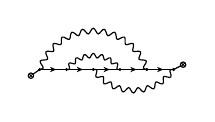
\begin{tikzpicture}[x=0.340cm, y=0.340cm, line width=0.420pt, baseline={([yshift=-0.6ex]0,0)}]
  \draw (-0.500,0.000) -- (0.500,0.000);
  \fill (0.119,0.000) -- (-0.119,0.102) -- (-0.042,0.000) -- (-0.119,-0.102) -- cycle;
  \draw (-1.500,0.000) -- (-0.500,0.000);
  \fill (-0.881,0.000) -- (-1.119,0.102) -- (-1.042,0.000) -- (-1.119,-0.102) -- cycle;
  \draw (0.500,0.000) -- (1.500,0.000);
  \fill (1.119,0.000) -- (0.881,0.102) -- (0.958,0.000) -- (0.881,-0.102) -- cycle;
  \draw (-2.500,0.000) -- (-1.500,0.000);
  \fill (-1.881,0.000) -- (-2.119,0.102) -- (-2.042,0.000) -- (-2.119,-0.102) -- cycle;
  \draw (1.500,0.000) -- (2.500,0.000);
  \fill (2.119,0.000) -- (1.881,0.102) -- (1.958,0.000) -- (1.881,-0.102) -- cycle;
  \draw plot[smooth, tension=0.7] coordinates {(0.500,0.000) (0.431,-0.003) (0.390,0.012) (0.385,0.055) (0.402,0.122) (0.417,0.190) (0.404,0.236) (0.358,0.247) (0.290,0.230) (0.224,0.210) (0.180,0.214) (0.164,0.254) (0.165,0.323) (0.161,0.393) (0.138,0.434) (0.090,0.433) (0.029,0.400) (-0.030,0.363) (-0.073,0.356) (-0.099,0.391) (-0.116,0.458) (-0.137,0.525) (-0.170,0.559) (-0.216,0.546) (-0.267,0.498) (-0.315,0.448) (-0.355,0.429) (-0.389,0.457) (-0.422,0.518) (-0.459,0.577) (-0.500,0.601) (-0.541,0.577) (-0.578,0.518) (-0.611,0.457) (-0.645,0.429) (-0.685,0.448) (-0.733,0.498) (-0.784,0.546) (-0.830,0.559) (-0.863,0.525) (-0.884,0.458) (-0.901,0.391) (-0.927,0.356) (-0.970,0.363) (-1.029,0.400) (-1.090,0.433) (-1.138,0.434) (-1.161,0.393) (-1.165,0.323) (-1.164,0.254) (-1.180,0.214) (-1.224,0.210) (-1.290,0.230) (-1.358,0.247) (-1.404,0.236) (-1.417,0.190) (-1.402,0.122) (-1.385,0.055) (-1.390,0.012) (-1.431,-0.003) (-1.500,0.000)};
  \draw plot[smooth, tension=0.7] coordinates {(-0.500,0.000) (-0.418,0.003) (-0.369,-0.015) (-0.364,-0.067) (-0.386,-0.146) (-0.406,-0.226) (-0.394,-0.281) (-0.340,-0.295) (-0.259,-0.279) (-0.179,-0.260) (-0.127,-0.268) (-0.111,-0.318) (-0.118,-0.399) (-0.121,-0.482) (-0.098,-0.533) (-0.042,-0.537) (0.034,-0.505) (0.108,-0.470) (0.160,-0.467) (0.186,-0.513) (0.196,-0.594) (0.209,-0.676) (0.242,-0.721) (0.298,-0.713) (0.366,-0.667) (0.431,-0.618) (0.482,-0.605) (0.516,-0.644) (0.542,-0.722) (0.572,-0.799) (0.613,-0.837) (0.666,-0.818) (0.724,-0.759) (0.778,-0.698) (0.825,-0.675) (0.867,-0.707) (0.908,-0.778) (0.952,-0.847) (1.000,-0.876) (1.048,-0.847) (1.092,-0.778) (1.133,-0.707) (1.175,-0.675) (1.222,-0.698) (1.276,-0.759) (1.334,-0.818) (1.387,-0.837) (1.428,-0.799) (1.458,-0.722) (1.484,-0.644) (1.518,-0.605) (1.569,-0.618) (1.634,-0.667) (1.702,-0.713) (1.758,-0.721) (1.791,-0.676) (1.804,-0.594) (1.814,-0.513) (1.840,-0.467) (1.892,-0.470) (1.966,-0.505) (2.042,-0.537) (2.098,-0.533) (2.121,-0.482) (2.118,-0.399) (2.111,-0.318) (2.127,-0.268) (2.179,-0.260) (2.259,-0.279) (2.340,-0.295) (2.394,-0.281) (2.406,-0.226) (2.386,-0.146) (2.364,-0.067) (2.369,-0.015) (2.418,0.003) (2.500,0.000)};
  \draw plot[smooth, tension=0.7] coordinates {(1.500,0.000) (1.417,0.022) (1.372,0.055) (1.383,0.110) (1.430,0.182) (1.474,0.257) (1.479,0.315) (1.430,0.347) (1.343,0.356) (1.257,0.362) (1.207,0.387) (1.207,0.442) (1.240,0.522) (1.271,0.604) (1.264,0.662) (1.210,0.684) (1.123,0.678) (1.037,0.668) (0.984,0.683) (0.974,0.737) (0.992,0.822) (1.006,0.908) (0.990,0.964) (0.932,0.976) (0.848,0.953) (0.765,0.928) (0.710,0.933) (0.690,0.984) (0.692,1.071) (0.691,1.158) (0.664,1.210) (0.605,1.211) (0.527,1.173) (0.450,1.133) (0.395,1.128) (0.366,1.175) (0.352,1.260) (0.335,1.346) (0.299,1.392) (0.241,1.382) (0.171,1.331) (0.103,1.277) (0.050,1.262) (0.012,1.303) (-0.017,1.384) (-0.050,1.465) (-0.094,1.504) (-0.149,1.483) (-0.208,1.420) (-0.265,1.355) (-0.315,1.330) (-0.359,1.363) (-0.403,1.438) (-0.450,1.511) (-0.500,1.541) (-0.550,1.511) (-0.597,1.438) (-0.641,1.363) (-0.685,1.330) (-0.735,1.355) (-0.792,1.420) (-0.851,1.483) (-0.906,1.504) (-0.950,1.465) (-0.983,1.384) (-1.012,1.303) (-1.050,1.262) (-1.103,1.277) (-1.171,1.331) (-1.241,1.382) (-1.299,1.392) (-1.335,1.346) (-1.352,1.260) (-1.366,1.175) (-1.395,1.128) (-1.450,1.133) (-1.527,1.173) (-1.605,1.211) (-1.664,1.210) (-1.691,1.158) (-1.692,1.071) (-1.690,0.984) (-1.710,0.933) (-1.765,0.928) (-1.848,0.953) (-1.932,0.976) (-1.990,0.964) (-2.006,0.908) (-1.992,0.822) (-1.974,0.737) (-1.984,0.683) (-2.037,0.668) (-2.123,0.678) (-2.210,0.684) (-2.264,0.662) (-2.271,0.604) (-2.240,0.522) (-2.207,0.442) (-2.207,0.387) (-2.257,0.362) (-2.343,0.356) (-2.430,0.347) (-2.479,0.315) (-2.474,0.257) (-2.430,0.182) (-2.383,0.110) (-2.372,0.055) (-2.417,0.022) (-2.500,0.000)};
  \draw (-2.500,0.000) -- (-2.828,-0.230);
  \draw[fill=white] (-2.828,-0.230) circle (0.100);
  \draw[line width=0.298pt] (-2.758,-0.160) -- (-2.898,-0.300) (-2.758,-0.300) -- (-2.898,-0.160);
  \draw (2.500,0.000) -- (2.857,0.181);
  \draw[fill=white] (2.857,0.181) circle (0.100);
  \draw[line width=0.298pt] (2.927,0.251) -- (2.787,0.111) (2.927,0.111) -- (2.787,0.251);
  \fill (0.500,0.000) circle (0.064);
  \fill (-0.500,0.000) circle (0.064);
  \fill (1.500,0.000) circle (0.064);
  \fill (-1.500,0.000) circle (0.064);
  \fill (2.500,0.000) circle (0.064);
  \fill (-2.500,0.000) circle (0.064);
\end{tikzpicture}}
\diagramgap
\mbox{$\displaystyle +\,$\,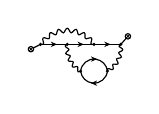
\begin{tikzpicture}[x=0.340cm, y=0.340cm, line width=0.420pt, baseline={([yshift=-0.6ex]0,0)}]
  \draw (1.000,-1.000) arc[start angle=353.974, end angle=186.026, radius=0.503];
  \fill (0.381,-1.450) -- (0.619,-1.552) -- (0.542,-1.450) -- (0.619,-1.348) -- cycle;
  \draw (0.000,-1.000) arc[start angle=173.974, end angle=6.026, radius=0.503];
  \fill (0.619,-0.550) -- (0.381,-0.448) -- (0.458,-0.550) -- (0.381,-0.652) -- cycle;
  \draw (-0.500,0.000) -- (0.500,0.000);
  \fill (0.119,0.000) -- (-0.119,0.102) -- (-0.042,0.000) -- (-0.119,-0.102) -- cycle;
  \draw (-1.500,0.000) -- (-0.500,0.000);
  \fill (-0.881,0.000) -- (-1.119,0.102) -- (-1.042,0.000) -- (-1.119,-0.102) -- cycle;
  \draw (0.500,0.000) -- (1.500,0.000);
  \fill (1.119,0.000) -- (0.881,0.102) -- (0.958,0.000) -- (0.881,-0.102) -- cycle;
  \draw plot[smooth, tension=0.7] coordinates {(0.000,-1.000) (-0.054,-1.025) (-0.094,-1.023) (-0.111,-0.987) (-0.110,-0.928) (-0.106,-0.870) (-0.117,-0.835) (-0.153,-0.829) (-0.210,-0.842) (-0.268,-0.852) (-0.307,-0.840) (-0.314,-0.800) (-0.298,-0.743) (-0.278,-0.689) (-0.280,-0.652) (-0.313,-0.637) (-0.371,-0.634) (-0.430,-0.629) (-0.464,-0.607) (-0.461,-0.567) (-0.430,-0.517) (-0.397,-0.469) (-0.389,-0.433) (-0.418,-0.409) (-0.473,-0.392) (-0.529,-0.371) (-0.556,-0.341) (-0.542,-0.304) (-0.499,-0.263) (-0.455,-0.225) (-0.438,-0.193) (-0.459,-0.163) (-0.508,-0.131) (-0.556,-0.097) (-0.575,-0.061) (-0.552,-0.028) (-0.500,0.000)};
  \draw plot[smooth, tension=0.7] coordinates {(1.000,-1.000) (1.003,-0.942) (1.019,-0.908) (1.056,-0.908) (1.110,-0.928) (1.167,-0.945) (1.206,-0.938) (1.219,-0.900) (1.210,-0.842) (1.198,-0.785) (1.204,-0.748) (1.240,-0.738) (1.298,-0.743) (1.357,-0.746) (1.393,-0.729) (1.395,-0.688) (1.371,-0.634) (1.345,-0.583) (1.341,-0.546) (1.373,-0.526) (1.430,-0.517) (1.488,-0.503) (1.519,-0.477) (1.510,-0.438) (1.473,-0.392) (1.434,-0.349) (1.421,-0.314) (1.447,-0.287) (1.499,-0.263) (1.551,-0.235) (1.574,-0.202) (1.556,-0.166) (1.508,-0.131) (1.459,-0.100) (1.438,-0.070) (1.455,-0.037) (1.500,0.000)};
  \draw plot[smooth, tension=0.7] coordinates {(0.500,0.000) (0.431,-0.003) (0.390,0.012) (0.385,0.055) (0.402,0.122) (0.417,0.190) (0.404,0.236) (0.358,0.247) (0.290,0.230) (0.224,0.210) (0.180,0.214) (0.164,0.254) (0.165,0.323) (0.161,0.393) (0.138,0.434) (0.090,0.433) (0.029,0.400) (-0.030,0.363) (-0.073,0.356) (-0.099,0.391) (-0.116,0.458) (-0.137,0.525) (-0.170,0.559) (-0.216,0.546) (-0.267,0.498) (-0.315,0.448) (-0.355,0.429) (-0.389,0.457) (-0.422,0.518) (-0.459,0.577) (-0.500,0.601) (-0.541,0.577) (-0.578,0.518) (-0.611,0.457) (-0.645,0.429) (-0.685,0.448) (-0.733,0.498) (-0.784,0.546) (-0.830,0.559) (-0.863,0.525) (-0.884,0.458) (-0.901,0.391) (-0.927,0.356) (-0.970,0.363) (-1.029,0.400) (-1.090,0.433) (-1.138,0.434) (-1.161,0.393) (-1.165,0.323) (-1.164,0.254) (-1.180,0.214) (-1.224,0.210) (-1.290,0.230) (-1.358,0.247) (-1.404,0.236) (-1.417,0.190) (-1.402,0.122) (-1.385,0.055) (-1.390,0.012) (-1.431,-0.003) (-1.500,0.000)};
  \draw (-1.500,0.000) -- (-1.857,-0.181);
  \draw[fill=white] (-1.857,-0.181) circle (0.100);
  \draw[line width=0.298pt] (-1.787,-0.111) -- (-1.927,-0.251) (-1.787,-0.251) -- (-1.927,-0.111);
  \draw (1.500,0.000) -- (1.766,0.299);
  \draw[fill=white] (1.766,0.299) circle (0.100);
  \draw[line width=0.298pt] (1.836,0.369) -- (1.696,0.229) (1.836,0.229) -- (1.696,0.369);
  \fill (0.000,-1.000) circle (0.064);
  \fill (1.000,-1.000) circle (0.064);
  \fill (0.500,0.000) circle (0.064);
  \fill (-0.500,0.000) circle (0.064);
  \fill (1.500,0.000) circle (0.064);
  \fill (-1.500,0.000) circle (0.064);
\end{tikzpicture}}
\diagramgap
\mbox{$\displaystyle +\,$\,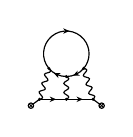
\begin{tikzpicture}[x=0.340cm, y=0.340cm, line width=0.420pt, baseline={([yshift=-0.6ex]0,0)}]
  \draw (0.651,1.154) arc[start angle=320.000, end angle=270.000, radius=0.850];
  \fill (0.251,0.879) -- (0.511,0.888) -- (0.397,0.947) -- (0.424,1.073) -- cycle;
  \draw (-0.651,1.154) arc[start angle=220.000, end angle=-40.000, radius=0.850];
  \fill (0.119,2.550) -- (-0.119,2.652) -- (-0.042,2.550) -- (-0.119,2.448) -- cycle;
  \draw (0.000,0.850) arc[start angle=270.000, end angle=220.000, radius=0.850];
  \fill (-0.467,0.980) -- (-0.294,0.787) -- (-0.321,0.912) -- (-0.208,0.972) -- cycle;
  \draw (-1.000,0.000) -- (0.000,0.000);
  \fill (-0.381,0.000) -- (-0.619,0.102) -- (-0.542,0.000) -- (-0.619,-0.102) -- cycle;
  \draw (0.000,0.000) -- (1.000,0.000);
  \fill (0.619,0.000) -- (0.381,0.102) -- (0.458,0.000) -- (0.381,-0.102) -- cycle;
  \draw plot[smooth, tension=0.7] coordinates {(0.000,0.850) (0.065,0.808) (0.092,0.765) (0.065,0.722) (0.000,0.680) (-0.065,0.638) (-0.092,0.595) (-0.065,0.552) (0.000,0.510) (0.065,0.467) (0.092,0.425) (0.065,0.382) (0.000,0.340) (-0.065,0.298) (-0.092,0.255) (-0.065,0.213) (0.000,0.170) (0.065,0.127) (0.092,0.085) (0.065,0.042) (0.000,0.000)};
  \draw plot[smooth, tension=0.7] coordinates {(0.651,1.154) (0.727,1.131) (0.765,1.098) (0.751,1.049) (0.701,0.989) (0.651,0.929) (0.637,0.880) (0.675,0.846) (0.751,0.824) (0.826,0.802) (0.865,0.769) (0.851,0.719) (0.801,0.659) (0.750,0.599) (0.737,0.550) (0.775,0.517) (0.850,0.494) (0.926,0.472) (0.964,0.439) (0.951,0.390) (0.900,0.330) (0.850,0.269) (0.836,0.220) (0.875,0.187) (0.950,0.165) (1.026,0.143) (1.064,0.109) (1.050,0.060) (1.000,0.000)};
  \draw plot[smooth, tension=0.7] coordinates {(-0.651,1.154) (-0.601,1.093) (-0.587,1.044) (-0.626,1.011) (-0.701,0.989) (-0.776,0.967) (-0.815,0.933) (-0.801,0.884) (-0.751,0.824) (-0.700,0.764) (-0.687,0.715) (-0.725,0.681) (-0.801,0.659) (-0.876,0.637) (-0.915,0.604) (-0.901,0.555) (-0.850,0.494) (-0.800,0.434) (-0.786,0.385) (-0.825,0.352) (-0.900,0.330) (-0.976,0.307) (-1.014,0.274) (-1.001,0.225) (-0.950,0.165) (-0.900,0.105) (-0.886,0.055) (-0.925,0.022) (-1.000,0.000)};
  \draw (-1.000,0.000) -- (-1.321,-0.238);
  \draw[fill=white] (-1.321,-0.238) circle (0.100);
  \draw[line width=0.298pt] (-1.251,-0.168) -- (-1.391,-0.308) (-1.251,-0.308) -- (-1.391,-0.168);
  \draw (1.000,0.000) -- (1.321,-0.238);
  \draw[fill=white] (1.321,-0.238) circle (0.100);
  \draw[line width=0.298pt] (1.391,-0.168) -- (1.251,-0.308) (1.391,-0.308) -- (1.251,-0.168);
  \fill (0.000,0.850) circle (0.064);
  \fill (0.651,1.154) circle (0.064);
  \fill (-0.651,1.154) circle (0.064);
  \fill (0.000,0.000) circle (0.064);
  \fill (1.000,0.000) circle (0.064);
  \fill (-1.000,0.000) circle (0.064);
\end{tikzpicture}}
\diagramgap
\mbox{$\displaystyle +\,$\,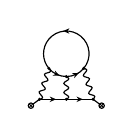
\begin{tikzpicture}[x=0.340cm, y=0.340cm, line width=0.420pt, baseline={([yshift=-0.6ex]0,0)}]
  \draw (-0.651,1.154) arc[start angle=220.000, end angle=270.000, radius=0.850];
  \fill (-0.251,0.879) -- (-0.424,1.073) -- (-0.397,0.947) -- (-0.511,0.888) -- cycle;
  \draw (0.000,0.850) arc[start angle=270.000, end angle=320.000, radius=0.850];
  \fill (0.467,0.980) -- (0.208,0.972) -- (0.321,0.912) -- (0.294,0.787) -- cycle;
  \draw (0.651,1.154) arc[start angle=320.000, end angle=580.000, radius=0.850];
  \fill (-0.119,2.550) -- (0.119,2.448) -- (0.042,2.550) -- (0.119,2.652) -- cycle;
  \draw (-1.000,0.000) -- (0.000,0.000);
  \fill (-0.381,0.000) -- (-0.619,0.102) -- (-0.542,0.000) -- (-0.619,-0.102) -- cycle;
  \draw (0.000,0.000) -- (1.000,0.000);
  \fill (0.619,0.000) -- (0.381,0.102) -- (0.458,0.000) -- (0.381,-0.102) -- cycle;
  \draw plot[smooth, tension=0.7] coordinates {(0.000,0.850) (0.065,0.808) (0.092,0.765) (0.065,0.722) (0.000,0.680) (-0.065,0.638) (-0.092,0.595) (-0.065,0.552) (0.000,0.510) (0.065,0.467) (0.092,0.425) (0.065,0.382) (0.000,0.340) (-0.065,0.298) (-0.092,0.255) (-0.065,0.213) (0.000,0.170) (0.065,0.127) (0.092,0.085) (0.065,0.042) (0.000,0.000)};
  \draw plot[smooth, tension=0.7] coordinates {(0.651,1.154) (0.727,1.131) (0.765,1.098) (0.751,1.049) (0.701,0.989) (0.651,0.929) (0.637,0.880) (0.675,0.846) (0.751,0.824) (0.826,0.802) (0.865,0.769) (0.851,0.719) (0.801,0.659) (0.750,0.599) (0.737,0.550) (0.775,0.517) (0.850,0.494) (0.926,0.472) (0.964,0.439) (0.951,0.390) (0.900,0.330) (0.850,0.269) (0.836,0.220) (0.875,0.187) (0.950,0.165) (1.026,0.143) (1.064,0.109) (1.050,0.060) (1.000,0.000)};
  \draw plot[smooth, tension=0.7] coordinates {(-0.651,1.154) (-0.601,1.093) (-0.587,1.044) (-0.626,1.011) (-0.701,0.989) (-0.776,0.967) (-0.815,0.933) (-0.801,0.884) (-0.751,0.824) (-0.700,0.764) (-0.687,0.715) (-0.725,0.681) (-0.801,0.659) (-0.876,0.637) (-0.915,0.604) (-0.901,0.555) (-0.850,0.494) (-0.800,0.434) (-0.786,0.385) (-0.825,0.352) (-0.900,0.330) (-0.976,0.307) (-1.014,0.274) (-1.001,0.225) (-0.950,0.165) (-0.900,0.105) (-0.886,0.055) (-0.925,0.022) (-1.000,0.000)};
  \draw (-1.000,0.000) -- (-1.321,-0.238);
  \draw[fill=white] (-1.321,-0.238) circle (0.100);
  \draw[line width=0.298pt] (-1.251,-0.168) -- (-1.391,-0.308) (-1.251,-0.308) -- (-1.391,-0.168);
  \draw (1.000,0.000) -- (1.321,-0.238);
  \draw[fill=white] (1.321,-0.238) circle (0.100);
  \draw[line width=0.298pt] (1.391,-0.168) -- (1.251,-0.308) (1.391,-0.308) -- (1.251,-0.168);
  \fill (0.000,0.850) circle (0.064);
  \fill (0.651,1.154) circle (0.064);
  \fill (-0.651,1.154) circle (0.064);
  \fill (0.000,0.000) circle (0.064);
  \fill (1.000,0.000) circle (0.064);
  \fill (-1.000,0.000) circle (0.064);
\end{tikzpicture}}
\diagramgap
\mbox{$\displaystyle -\,$\,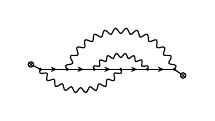
\begin{tikzpicture}[x=0.340cm, y=0.340cm, line width=0.420pt, baseline={([yshift=-0.6ex]0,0)}]
  \draw (-1.500,0.000) -- (-0.500,0.000);
  \fill (-0.881,0.000) -- (-1.119,0.102) -- (-1.042,0.000) -- (-1.119,-0.102) -- cycle;
  \draw (-0.500,0.000) -- (0.500,0.000);
  \fill (0.119,0.000) -- (-0.119,0.102) -- (-0.042,0.000) -- (-0.119,-0.102) -- cycle;
  \draw (0.500,0.000) -- (1.500,0.000);
  \fill (1.119,0.000) -- (0.881,0.102) -- (0.958,0.000) -- (0.881,-0.102) -- cycle;
  \draw (-2.500,0.000) -- (-1.500,0.000);
  \fill (-1.881,0.000) -- (-2.119,0.102) -- (-2.042,0.000) -- (-2.119,-0.102) -- cycle;
  \draw (1.500,0.000) -- (2.500,0.000);
  \fill (2.119,0.000) -- (1.881,0.102) -- (1.958,0.000) -- (1.881,-0.102) -- cycle;
  \draw plot[smooth, tension=0.7] coordinates {(-0.500,0.000) (-0.523,0.066) (-0.517,0.113) (-0.472,0.130) (-0.402,0.122) (-0.334,0.110) (-0.292,0.119) (-0.281,0.162) (-0.290,0.230) (-0.296,0.300) (-0.277,0.344) (-0.230,0.349) (-0.165,0.323) (-0.102,0.295) (-0.058,0.293) (-0.037,0.331) (-0.029,0.400) (-0.016,0.469) (0.012,0.507) (0.059,0.499) (0.116,0.458) (0.170,0.415) (0.212,0.402) (0.242,0.434) (0.267,0.498) (0.296,0.561) (0.334,0.591) (0.378,0.572) (0.422,0.518) (0.463,0.462) (0.500,0.439) (0.537,0.462) (0.578,0.518) (0.622,0.572) (0.666,0.591) (0.704,0.561) (0.733,0.498) (0.758,0.434) (0.788,0.402) (0.830,0.415) (0.884,0.458) (0.941,0.499) (0.988,0.507) (1.016,0.469) (1.029,0.400) (1.037,0.331) (1.058,0.293) (1.102,0.295) (1.165,0.323) (1.230,0.349) (1.277,0.344) (1.296,0.300) (1.290,0.230) (1.281,0.162) (1.292,0.119) (1.334,0.110) (1.402,0.122) (1.472,0.130) (1.517,0.113) (1.523,0.066) (1.500,0.000)};
  \draw plot[smooth, tension=0.7] coordinates {(0.500,0.000) (0.528,-0.078) (0.521,-0.133) (0.469,-0.154) (0.386,-0.146) (0.305,-0.135) (0.255,-0.148) (0.244,-0.199) (0.259,-0.279) (0.270,-0.361) (0.252,-0.414) (0.197,-0.424) (0.118,-0.399) (0.041,-0.372) (-0.012,-0.375) (-0.032,-0.423) (-0.034,-0.505) (-0.039,-0.587) (-0.067,-0.636) (-0.123,-0.634) (-0.196,-0.594) (-0.266,-0.552) (-0.318,-0.544) (-0.348,-0.587) (-0.366,-0.667) (-0.388,-0.747) (-0.425,-0.788) (-0.479,-0.775) (-0.542,-0.722) (-0.603,-0.667) (-0.652,-0.649) (-0.690,-0.685) (-0.724,-0.759) (-0.761,-0.833) (-0.806,-0.866) (-0.856,-0.843) (-0.908,-0.778) (-0.955,-0.711) (-1.000,-0.684) (-1.045,-0.711) (-1.092,-0.778) (-1.144,-0.843) (-1.194,-0.866) (-1.239,-0.833) (-1.276,-0.759) (-1.310,-0.685) (-1.348,-0.649) (-1.397,-0.667) (-1.458,-0.722) (-1.521,-0.775) (-1.575,-0.788) (-1.612,-0.747) (-1.634,-0.667) (-1.652,-0.587) (-1.682,-0.544) (-1.734,-0.552) (-1.804,-0.594) (-1.877,-0.634) (-1.933,-0.636) (-1.961,-0.587) (-1.966,-0.505) (-1.968,-0.423) (-1.988,-0.375) (-2.041,-0.372) (-2.118,-0.399) (-2.197,-0.424) (-2.252,-0.414) (-2.270,-0.361) (-2.259,-0.279) (-2.244,-0.199) (-2.255,-0.148) (-2.305,-0.135) (-2.386,-0.146) (-2.469,-0.154) (-2.521,-0.133) (-2.528,-0.078) (-2.500,0.000)};
  \draw plot[smooth, tension=0.7] coordinates {(-1.500,0.000) (-1.551,0.070) (-1.562,0.128) (-1.515,0.164) (-1.430,0.182) (-1.345,0.196) (-1.298,0.225) (-1.303,0.280) (-1.343,0.356) (-1.381,0.435) (-1.380,0.494) (-1.328,0.521) (-1.240,0.522) (-1.154,0.520) (-1.103,0.540) (-1.098,0.595) (-1.123,0.678) (-1.146,0.762) (-1.134,0.819) (-1.078,0.836) (-0.992,0.822) (-0.907,0.804) (-0.853,0.814) (-0.838,0.867) (-0.848,0.953) (-0.855,1.040) (-0.833,1.094) (-0.774,1.101) (-0.692,1.071) (-0.613,1.038) (-0.557,1.038) (-0.533,1.087) (-0.527,1.173) (-0.517,1.260) (-0.486,1.309) (-0.427,1.305) (-0.352,1.260) (-0.280,1.213) (-0.226,1.203) (-0.192,1.247) (-0.171,1.331) (-0.145,1.414) (-0.105,1.457) (-0.048,1.442) (0.017,1.384) (0.079,1.324) (0.131,1.304) (0.172,1.342) (0.208,1.420) (0.249,1.497) (0.296,1.532) (0.349,1.506) (0.403,1.438) (0.453,1.368) (0.500,1.339) (0.547,1.368) (0.597,1.438) (0.651,1.506) (0.704,1.532) (0.751,1.497) (0.792,1.420) (0.828,1.342) (0.869,1.304) (0.921,1.324) (0.983,1.384) (1.048,1.442) (1.105,1.457) (1.145,1.414) (1.171,1.331) (1.192,1.247) (1.226,1.203) (1.280,1.213) (1.352,1.260) (1.427,1.305) (1.486,1.309) (1.517,1.260) (1.527,1.173) (1.533,1.087) (1.557,1.038) (1.613,1.038) (1.692,1.071) (1.774,1.101) (1.833,1.094) (1.855,1.040) (1.848,0.953) (1.838,0.867) (1.853,0.814) (1.907,0.804) (1.992,0.822) (2.078,0.836) (2.134,0.819) (2.146,0.762) (2.123,0.678) (2.098,0.595) (2.103,0.540) (2.154,0.520) (2.240,0.522) (2.328,0.521) (2.380,0.494) (2.381,0.435) (2.343,0.356) (2.303,0.280) (2.298,0.225) (2.345,0.196) (2.430,0.182) (2.515,0.164) (2.562,0.128) (2.551,0.070) (2.500,0.000)};
  \draw (-2.500,0.000) -- (-2.857,0.181);
  \draw[fill=white] (-2.857,0.181) circle (0.100);
  \draw[line width=0.298pt] (-2.787,0.251) -- (-2.927,0.111) (-2.787,0.111) -- (-2.927,0.251);
  \draw (2.500,0.000) -- (2.828,-0.230);
  \draw[fill=white] (2.828,-0.230) circle (0.100);
  \draw[line width=0.298pt] (2.898,-0.160) -- (2.758,-0.300) (2.898,-0.300) -- (2.758,-0.160);
  \fill (-0.500,0.000) circle (0.064);
  \fill (0.500,0.000) circle (0.064);
  \fill (1.500,0.000) circle (0.064);
  \fill (-1.500,0.000) circle (0.064);
  \fill (2.500,0.000) circle (0.064);
  \fill (-2.500,0.000) circle (0.064);
\end{tikzpicture}}
\diagramgap
\mbox{$\displaystyle +\,$\,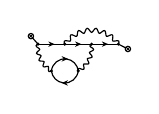
\begin{tikzpicture}[x=0.340cm, y=0.340cm, line width=0.420pt, baseline={([yshift=-0.6ex]0,0)}]
  \draw (-1.000,-1.000) arc[start angle=173.974, end angle=6.026, radius=0.503];
  \fill (-0.381,-0.550) -- (-0.619,-0.448) -- (-0.542,-0.550) -- (-0.619,-0.652) -- cycle;
  \draw (0.000,-1.000) arc[start angle=353.974, end angle=186.026, radius=0.503];
  \fill (-0.619,-1.450) -- (-0.381,-1.552) -- (-0.458,-1.450) -- (-0.381,-1.348) -- cycle;
  \draw (-0.500,0.000) -- (0.500,0.000);
  \fill (0.119,0.000) -- (-0.119,0.102) -- (-0.042,0.000) -- (-0.119,-0.102) -- cycle;
  \draw (-1.500,0.000) -- (-0.500,0.000);
  \fill (-0.881,0.000) -- (-1.119,0.102) -- (-1.042,0.000) -- (-1.119,-0.102) -- cycle;
  \draw (0.500,0.000) -- (1.500,0.000);
  \fill (1.119,0.000) -- (0.881,0.102) -- (0.958,0.000) -- (0.881,-0.102) -- cycle;
  \draw plot[smooth, tension=0.7] coordinates {(0.000,-1.000) (0.003,-0.942) (0.019,-0.908) (0.056,-0.908) (0.110,-0.928) (0.167,-0.945) (0.206,-0.938) (0.219,-0.900) (0.210,-0.842) (0.198,-0.785) (0.204,-0.748) (0.240,-0.738) (0.298,-0.743) (0.357,-0.746) (0.393,-0.729) (0.395,-0.688) (0.371,-0.634) (0.345,-0.583) (0.341,-0.546) (0.373,-0.526) (0.430,-0.517) (0.488,-0.503) (0.519,-0.477) (0.510,-0.438) (0.473,-0.392) (0.434,-0.349) (0.421,-0.314) (0.447,-0.287) (0.499,-0.263) (0.551,-0.235) (0.574,-0.202) (0.556,-0.166) (0.508,-0.131) (0.459,-0.100) (0.438,-0.070) (0.455,-0.037) (0.500,0.000)};
  \draw plot[smooth, tension=0.7] coordinates {(-1.000,-1.000) (-1.054,-1.025) (-1.094,-1.023) (-1.111,-0.987) (-1.110,-0.928) (-1.106,-0.870) (-1.117,-0.835) (-1.153,-0.829) (-1.210,-0.842) (-1.268,-0.852) (-1.307,-0.840) (-1.314,-0.800) (-1.298,-0.743) (-1.278,-0.689) (-1.280,-0.652) (-1.313,-0.637) (-1.371,-0.634) (-1.430,-0.629) (-1.464,-0.607) (-1.461,-0.567) (-1.430,-0.517) (-1.397,-0.469) (-1.389,-0.433) (-1.418,-0.409) (-1.473,-0.392) (-1.529,-0.371) (-1.556,-0.341) (-1.542,-0.304) (-1.499,-0.263) (-1.455,-0.225) (-1.438,-0.193) (-1.459,-0.163) (-1.508,-0.131) (-1.556,-0.097) (-1.575,-0.061) (-1.552,-0.028) (-1.500,0.000)};
  \draw plot[smooth, tension=0.7] coordinates {(-0.500,0.000) (-0.523,0.066) (-0.517,0.113) (-0.472,0.130) (-0.402,0.122) (-0.334,0.110) (-0.292,0.119) (-0.281,0.162) (-0.290,0.230) (-0.296,0.300) (-0.277,0.344) (-0.230,0.349) (-0.165,0.323) (-0.102,0.295) (-0.058,0.293) (-0.037,0.331) (-0.029,0.400) (-0.016,0.469) (0.012,0.507) (0.059,0.499) (0.116,0.458) (0.170,0.415) (0.212,0.402) (0.242,0.434) (0.267,0.498) (0.296,0.561) (0.334,0.591) (0.378,0.572) (0.422,0.518) (0.463,0.462) (0.500,0.439) (0.537,0.462) (0.578,0.518) (0.622,0.572) (0.666,0.591) (0.704,0.561) (0.733,0.498) (0.758,0.434) (0.788,0.402) (0.830,0.415) (0.884,0.458) (0.941,0.499) (0.988,0.507) (1.016,0.469) (1.029,0.400) (1.037,0.331) (1.058,0.293) (1.102,0.295) (1.165,0.323) (1.230,0.349) (1.277,0.344) (1.296,0.300) (1.290,0.230) (1.281,0.162) (1.292,0.119) (1.334,0.110) (1.402,0.122) (1.472,0.130) (1.517,0.113) (1.523,0.066) (1.500,0.000)};
  \draw (-1.500,0.000) -- (-1.766,0.299);
  \draw[fill=white] (-1.766,0.299) circle (0.100);
  \draw[line width=0.298pt] (-1.696,0.369) -- (-1.836,0.229) (-1.696,0.229) -- (-1.836,0.369);
  \draw (1.500,0.000) -- (1.857,-0.181);
  \draw[fill=white] (1.857,-0.181) circle (0.100);
  \draw[line width=0.298pt] (1.927,-0.111) -- (1.787,-0.251) (1.927,-0.251) -- (1.787,-0.111);
  \fill (0.000,-1.000) circle (0.064);
  \fill (-1.000,-1.000) circle (0.064);
  \fill (0.500,0.000) circle (0.064);
  \fill (-0.500,0.000) circle (0.064);
  \fill (1.500,0.000) circle (0.064);
  \fill (-1.500,0.000) circle (0.064);
\end{tikzpicture}}
\diagramgap
\mbox{$\displaystyle +\,\frac{1}{6}$\,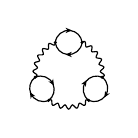
\begin{tikzpicture}[x=0.340cm, y=0.340cm, line width=0.420pt, baseline={([yshift=-0.6ex]0,0)}]
  \draw (0.500,1.155) arc[start angle=353.974, end angle=186.026, radius=0.503];
  \fill (-0.119,0.705) -- (0.119,0.603) -- (0.042,0.705) -- (0.119,0.807) -- cycle;
  \draw (-0.500,1.155) arc[start angle=173.974, end angle=6.026, radius=0.503];
  \fill (0.119,1.605) -- (-0.119,1.707) -- (-0.042,1.605) -- (-0.119,1.503) -- cycle;
  \draw (-0.750,-1.010) arc[start angle=293.974, end angle=126.026, radius=0.503];
  \fill (-1.449,-0.699) -- (-1.418,-0.957) -- (-1.369,-0.839) -- (-1.242,-0.855) -- cycle;
  \draw (-1.250,-0.144) arc[start angle=113.974, end angle=-53.974, radius=0.503];
  \fill (-0.551,-0.456) -- (-0.582,-0.198) -- (-0.631,-0.316) -- (-0.758,-0.300) -- cycle;
  \draw (0.750,-1.010) arc[start angle=233.974, end angle=66.026, radius=0.503];
  \fill (0.670,-0.249) -- (0.462,-0.405) -- (0.589,-0.389) -- (0.639,-0.507) -- cycle;
  \draw (1.250,-0.144) arc[start angle=53.974, end angle=-113.974, radius=0.503];
  \fill (1.330,-0.906) -- (1.538,-0.750) -- (1.411,-0.766) -- (1.361,-0.648) -- cycle;
  \draw plot[smooth, tension=0.7] coordinates {(-0.500,1.155) (-0.511,1.091) (-0.532,1.056) (-0.573,1.060) (-0.631,1.089) (-0.690,1.117) (-0.735,1.115) (-0.754,1.075) (-0.753,1.009) (-0.749,0.945) (-0.762,0.906) (-0.802,0.900) (-0.865,0.916) (-0.929,0.928) (-0.972,0.916) (-0.982,0.873) (-0.966,0.809) (-0.947,0.748) (-0.950,0.707) (-0.988,0.692) (-1.053,0.692) (-1.118,0.690) (-1.157,0.668) (-1.156,0.624) (-1.126,0.566) (-1.093,0.510) (-1.087,0.469) (-1.121,0.446) (-1.184,0.431) (-1.247,0.414) (-1.280,0.384) (-1.269,0.341) (-1.226,0.291) (-1.181,0.245) (-1.165,0.207) (-1.193,0.176) (-1.251,0.147) (-1.308,0.116) (-1.333,0.079) (-1.312,0.040) (-1.259,0.002) (-1.205,-0.033) (-1.181,-0.067) (-1.200,-0.103) (-1.250,-0.144)};
  \draw plot[smooth, tension=0.7] coordinates {(0.500,1.155) (0.556,1.189) (0.600,1.192) (0.624,1.155) (0.631,1.089) (0.634,1.025) (0.651,0.988) (0.693,0.987) (0.753,1.009) (0.815,1.029) (0.859,1.023) (0.874,0.981) (0.865,0.916) (0.853,0.852) (0.862,0.812) (0.902,0.801) (0.966,0.809) (1.031,0.815) (1.072,0.798) (1.076,0.753) (1.053,0.692) (1.027,0.633) (1.025,0.592) (1.062,0.573) (1.126,0.566) (1.191,0.556) (1.227,0.530) (1.221,0.485) (1.184,0.431) (1.145,0.380) (1.134,0.340) (1.165,0.313) (1.226,0.291) (1.286,0.267) (1.315,0.233) (1.299,0.191) (1.251,0.147) (1.201,0.107) (1.181,0.070) (1.205,0.037) (1.259,0.002) (1.312,-0.037) (1.332,-0.076) (1.307,-0.113) (1.250,-0.144)};
  \draw plot[smooth, tension=0.7] coordinates {(-0.750,-1.010) (-0.689,-0.988) (-0.648,-0.989) (-0.631,-1.026) (-0.628,-1.091) (-0.622,-1.156) (-0.598,-1.194) (-0.554,-1.191) (-0.498,-1.157) (-0.444,-1.121) (-0.404,-1.113) (-0.378,-1.145) (-0.360,-1.207) (-0.339,-1.269) (-0.307,-1.300) (-0.265,-1.287) (-0.218,-1.241) (-0.174,-1.194) (-0.137,-1.176) (-0.105,-1.202) (-0.073,-1.258) (-0.038,-1.313) (0.000,-1.336) (0.038,-1.313) (0.073,-1.258) (0.105,-1.202) (0.137,-1.176) (0.174,-1.194) (0.218,-1.241) (0.265,-1.287) (0.307,-1.300) (0.339,-1.269) (0.360,-1.207) (0.378,-1.145) (0.404,-1.113) (0.444,-1.121) (0.498,-1.157) (0.554,-1.191) (0.598,-1.194) (0.622,-1.156) (0.628,-1.091) (0.631,-1.026) (0.648,-0.989) (0.689,-0.988) (0.750,-1.010)};
  \fill (-0.500,1.155) circle (0.064);
  \fill (0.500,1.155) circle (0.064);
  \fill (-1.250,-0.144) circle (0.064);
  \fill (-0.750,-1.010) circle (0.064);
  \fill (1.250,-0.144) circle (0.064);
  \fill (0.750,-1.010) circle (0.064);
\end{tikzpicture}}
\diagramgap
\mbox{$\displaystyle +\,$\,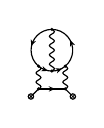
\begin{tikzpicture}[x=0.340cm, y=0.340cm, line width=0.420pt, baseline={([yshift=-0.6ex]0,0)}]
  \draw (0.500,0.850) arc[start angle=310.003, end angle=450.000, radius=0.778];
  \fill (0.690,1.824) -- (0.676,1.565) -- (0.745,1.673) -- (0.868,1.635) -- cycle;
  \draw (-0.500,0.850) arc[start angle=229.997, end angle=270.000, radius=0.778];
  \fill (-0.154,0.674) -- (-0.343,0.852) -- (-0.305,0.729) -- (-0.413,0.660) -- cycle;
  \draw (0.000,0.668) arc[start angle=270.000, end angle=310.003, radius=0.778];
  \fill (0.378,0.756) -- (0.119,0.770) -- (0.227,0.701) -- (0.189,0.578) -- cycle;
  \draw (0.000,2.224) arc[start angle=90.000, end angle=229.997, radius=0.778];
  \fill (-0.772,1.600) -- (-0.594,1.789) -- (-0.717,1.751) -- (-0.786,1.859) -- cycle;
  \draw (-0.500,0.000) -- (0.500,0.000);
  \fill (0.119,0.000) -- (-0.119,0.102) -- (-0.042,0.000) -- (-0.119,-0.102) -- cycle;
  \draw plot[smooth, tension=0.7] coordinates {(0.000,2.224) (0.066,2.180) (0.093,2.137) (0.066,2.094) (0.000,2.051) (-0.066,2.008) (-0.093,1.964) (-0.066,1.921) (0.000,1.878) (0.066,1.835) (0.093,1.792) (0.066,1.748) (0.000,1.705) (-0.066,1.662) (-0.093,1.619) (-0.066,1.575) (0.000,1.532) (0.066,1.489) (0.093,1.446) (0.066,1.403) (0.000,1.359) (-0.066,1.316) (-0.093,1.273) (-0.066,1.230) (0.000,1.187) (0.066,1.143) (0.093,1.100) (0.066,1.057) (0.000,1.014) (-0.066,0.970) (-0.093,0.927) (-0.066,0.884) (0.000,0.841) (0.066,0.798) (0.093,0.754) (0.066,0.711) (0.000,0.668)};
  \draw plot[smooth, tension=0.7] coordinates {(0.500,0.850) (0.565,0.808) (0.592,0.765) (0.565,0.722) (0.500,0.680) (0.435,0.638) (0.408,0.595) (0.435,0.552) (0.500,0.510) (0.565,0.468) (0.592,0.425) (0.565,0.382) (0.500,0.340) (0.435,0.298) (0.408,0.255) (0.435,0.213) (0.500,0.170) (0.565,0.127) (0.592,0.085) (0.565,0.042) (0.500,0.000)};
  \draw plot[smooth, tension=0.7] coordinates {(-0.500,0.850) (-0.435,0.808) (-0.408,0.765) (-0.435,0.723) (-0.500,0.680) (-0.565,0.638) (-0.592,0.595) (-0.565,0.553) (-0.500,0.510) (-0.435,0.468) (-0.408,0.425) (-0.435,0.383) (-0.500,0.340) (-0.565,0.298) (-0.592,0.255) (-0.565,0.213) (-0.500,0.170) (-0.435,0.127) (-0.408,0.085) (-0.435,0.042) (-0.500,0.000)};
  \draw (-0.500,0.000) -- (-0.783,-0.283);
  \draw[fill=white] (-0.783,-0.283) circle (0.100);
  \draw[line width=0.298pt] (-0.713,-0.213) -- (-0.853,-0.353) (-0.713,-0.353) -- (-0.853,-0.213);
  \draw (0.500,0.000) -- (0.783,-0.283);
  \draw[fill=white] (0.783,-0.283) circle (0.100);
  \draw[line width=0.298pt] (0.853,-0.213) -- (0.713,-0.353) (0.853,-0.353) -- (0.713,-0.213);
  \fill (0.000,2.224) circle (0.064);
  \fill (0.000,0.668) circle (0.064);
  \fill (0.500,0.850) circle (0.064);
  \fill (-0.500,0.850) circle (0.064);
  \fill (0.500,0.000) circle (0.064);
  \fill (-0.500,0.000) circle (0.064);
\end{tikzpicture}}
\diagramgap
\mbox{$\displaystyle -\,$\,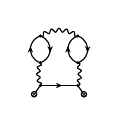
\begin{tikzpicture}[x=0.340cm, y=0.340cm, line width=0.420pt, baseline={([yshift=-0.6ex]0,0)}]
  \draw (0.700,0.850) arc[start angle=252.811, end angle=107.189, radius=0.523];
  \fill (0.331,1.469) -- (0.229,1.231) -- (0.331,1.308) -- (0.433,1.231) -- cycle;
  \draw (0.700,1.850) arc[start angle=72.811, end angle=-72.811, radius=0.523];
  \fill (1.069,1.231) -- (1.171,1.469) -- (1.069,1.392) -- (0.967,1.469) -- cycle;
  \draw (-0.700,0.850) arc[start angle=252.811, end angle=107.189, radius=0.523];
  \fill (-1.069,1.469) -- (-1.171,1.231) -- (-1.069,1.308) -- (-0.967,1.231) -- cycle;
  \draw (-0.700,1.850) arc[start angle=72.811, end angle=-72.811, radius=0.523];
  \fill (-0.331,1.231) -- (-0.229,1.469) -- (-0.331,1.392) -- (-0.433,1.469) -- cycle;
  \draw (-0.700,0.000) -- (0.700,0.000);
  \fill (0.119,0.000) -- (-0.119,0.102) -- (-0.042,0.000) -- (-0.119,-0.102) -- cycle;
  \draw plot[smooth, tension=0.7] coordinates {(0.700,1.850) (0.645,1.827) (0.607,1.827) (0.589,1.861) (0.585,1.921) (0.577,1.981) (0.554,2.015) (0.513,2.011) (0.462,1.978) (0.413,1.944) (0.376,1.935) (0.352,1.965) (0.334,2.022) (0.314,2.079) (0.284,2.107) (0.245,2.094) (0.202,2.052) (0.162,2.007) (0.127,1.991) (0.097,2.014) (0.068,2.066) (0.035,2.118) (0.000,2.139) (-0.035,2.118) (-0.068,2.066) (-0.097,2.014) (-0.127,1.991) (-0.162,2.007) (-0.202,2.052) (-0.245,2.094) (-0.284,2.107) (-0.314,2.079) (-0.334,2.022) (-0.352,1.965) (-0.376,1.935) (-0.413,1.944) (-0.462,1.978) (-0.513,2.011) (-0.554,2.015) (-0.577,1.981) (-0.585,1.921) (-0.589,1.861) (-0.607,1.827) (-0.645,1.827) (-0.700,1.850)};
  \draw plot[smooth, tension=0.7] coordinates {(0.700,0.850) (0.753,0.835) (0.781,0.810) (0.773,0.774) (0.737,0.732) (0.700,0.691) (0.688,0.658) (0.712,0.633) (0.762,0.610) (0.811,0.585) (0.834,0.555) (0.818,0.521) (0.774,0.487) (0.730,0.455) (0.711,0.425) (0.730,0.395) (0.774,0.363) (0.818,0.329) (0.834,0.295) (0.811,0.265) (0.762,0.240) (0.712,0.217) (0.688,0.192) (0.700,0.159) (0.737,0.118) (0.773,0.076) (0.781,0.040) (0.753,0.015) (0.700,0.000)};
  \draw plot[smooth, tension=0.7] coordinates {(-0.700,0.850) (-0.667,0.806) (-0.658,0.772) (-0.685,0.749) (-0.737,0.732) (-0.789,0.712) (-0.814,0.684) (-0.801,0.649) (-0.762,0.610) (-0.721,0.574) (-0.705,0.542) (-0.727,0.514) (-0.774,0.487) (-0.821,0.457) (-0.840,0.425) (-0.821,0.393) (-0.774,0.363) (-0.727,0.336) (-0.705,0.308) (-0.721,0.276) (-0.762,0.240) (-0.801,0.201) (-0.814,0.166) (-0.789,0.138) (-0.737,0.118) (-0.685,0.101) (-0.658,0.078) (-0.667,0.044) (-0.700,0.000)};
  \draw (-0.700,0.000) -- (-0.930,-0.327);
  \draw[fill=white] (-0.930,-0.327) circle (0.100);
  \draw[line width=0.298pt] (-0.860,-0.257) -- (-1.000,-0.397) (-0.860,-0.397) -- (-1.000,-0.257);
  \draw (0.700,0.000) -- (0.930,-0.327);
  \draw[fill=white] (0.930,-0.327) circle (0.100);
  \draw[line width=0.298pt] (1.000,-0.257) -- (0.860,-0.397) (1.000,-0.397) -- (0.860,-0.257);
  \fill (0.700,1.850) circle (0.064);
  \fill (-0.700,1.850) circle (0.064);
  \fill (0.700,0.850) circle (0.064);
  \fill (-0.700,0.850) circle (0.064);
  \fill (0.700,0.000) circle (0.064);
  \fill (-0.700,0.000) circle (0.064);
\end{tikzpicture}}
